\subsection{E4：结构（探索）}
\label{sec:e4}

阻断 LU 割中的走廊时，funnel 与 high 的预约影响集占比随随机种子波动（表~\ref{tab:e4}）。
方向上 funnel 更高（中位数 \(0.254\) 对 \(0.204\)，均值 \(0.244\) 对 \(0.229\)），
但\emph{两组取值高度重叠}:funnel 落在 \([0.180,0.309]\),high 落在
\([0.156,0.372]\)，后者的区间完全包含前者，且单个随机种子即可使方向反转
（随机种子 \(2024\) 上 high 的 \(0.372\) 高于 funnel 的 \(0.296\)）。
在五个随机种子、两个布局上，这一差距不足以支撑任何结论。
第~\ref{sec:e1}~节按繁忙走廊阻断协议在三个同规模布局上得到的
\(\mathrm{Cl}/|R|\) 亦落在 \EoneCloLo--\EoneCloHi 的窄带内，同样未能区分布局。

\textbf{外部布局用于区分负结果的成因。}
三张同规模布局同属哑铃一族，几何差异很小（见表~\ref{tab:e4pub}：节点数 \(9\)--\(11\)、
走廊数 \(8\)--\(12\),LU 割仅取 \(1\) 或 \(2\)）；「指标过粗」与
「算例几何差异不足」两种解释在这些布局上无法区分。第~\ref{sec:protocol}~节的
第二批算例用于区分二者（表~\ref{tab:e4pub}）。

\textbf{外部布局上的结果与预期方向相反。}
这批算例在路网几何上只有 \NPubNets\ 个独立样本（第~\ref{sec:protocol}~节），故只用于考察机器配置这一维。
在\emph{同一张} \(4\times 4\) 路网上，只把机器台数与落位从 \(4\) 机换成 \(5\) 机，
影响集占比中位即由 \PubCloHi\ 落到 \PubCloLo，极差 \PubCloSpread；
同一张 \(5\times 5\) 路网上换三种机器配置（\(6\)、\(7\)、\(8\) 机），极差 \PubCloSpreadBig。
作为对比，\emph{逐参数同口径}的三张自建布局（三张\emph{不同}的路网）
的占比只落在 \SelfCloLo--\SelfCloHi，极差 \SelfCloSpread。
即\textbf{路网固定而机器配置变动时，影响集占比的变化幅度可以超过更换三张不同路网时的幅度}：
在 \(4\times 4\) 路网上约为四倍，在 \(5\times 5\) 路网上约为一点五倍。
这一比较并不对称：外部一侧同时改变了机器台数与落位，自建一侧只改变路网；且三张自建布局的几何差异很小，
\SelfCloSpread\ 只是「更换路网」幅度的\emph{下界}。因此它表明机器配置这一维不可忽略，
但不表明其效应大于路网几何。

\textbf{仅由路网决定的最小割无法解释影响集规模。}
在这 \NPubInst\ 个外部算例上，\textbf{LU 割恒为 \(2\)、漏斗占比恒为 \(0\)}：
两张路网都把装卸站放在网格角点，而四邻接网格的角点恰有两条出边，故该割值固定为 \(2\)；
同一工具集另附的那族布局（因允许对角移动未纳入本批）把装卸站放在网格边中点，出边数为 \(3\)。
\textbf{可见该指标在实际布局上只取少数几个由装卸站网格位置决定的离散值}，不随几何连续变化。
更重要的是，\textbf{这两个指标在上述全部变动中保持不变}，而被解释的量变化了
\PubCloSpread；取值恒定的指标无法解释一个变化的量。第三个指标（每节点走廊数）在整批上只取两个值（\(23/16\) 与
\(38/25\)），同样不足以解释组内的变化。

据此，\textbf{在这 \NPubInst\ 个外部算例与三张自建布局上，静态割不能解释影响集规模}。
这一族指标原本针对哑铃布局中可调的装卸站出口瓶颈而设计，在实际布局上退化为常量，不具备解释力。
替代方向由此指向需求侧：决定影响集规模的可能不是路网\emph{能}提供多少条通路，而是
\emph{需求的空间分布}；具体的候选量见第~\ref{sec:future}~节。
本节为探索性的负结果，不对应任何一项贡献。

\begin{table}[t]
\centering
\caption{E4 预约影响集占比 \(\mathrm{Cl}/|R|\)（阻断 LU 割中的走廊；随机种子 \(42,7,2024,99,123\)）。
本表算例为 \(12\) 工件 / \(8\) 机 / \(12\) 辆车、运输与加工时长比标定为 \(4.0\)。
\textbf{该口径与表~\ref{tab:e4pub} 不同}（后者为 \(8\) 工件 / \(4\) 机 / \(4\) 辆车、
比值 \(1.0\)、十个随机种子），两表虽共用 \texttt{funnel}/\texttt{high} 这两个布局名，
\emph{数值不可跨表比较}；表~\ref{tab:e4pub} 内部才是同口径对照。}
\label{tab:e4}
\small
\begin{tabular}{@{}lcccccc@{}}
\toprule
布局 & \(42\) & \(7\) & \(2024\) & \(99\) & \(123\) & 中位数 \\
\midrule
funnel & \(0.254\) & \(0.181\) & \(0.296\) & \(0.309\) & \(0.180\) & \(0.254\) \\
high & \(0.156\) & \(0.204\) & \(0.372\) & \(0.229\) & \(0.184\) & \(0.204\) \\
\bottomrule
\end{tabular}
\end{table}

\begin{table}[t]
\centering
\caption{E4 自建布局与外部布局的对照（阻断 LU 割中的走廊，十个随机种子；\(\mathrm{Cl}/|R|\) 取中位数）。
全表逐参数同口径，只差路网与机器配置。\textbf{外部算例只落在 \NPubNets\ 张路网上}
（\(\mathrm{N}_1\):\(4\times 4\) 去一条边；\(\mathrm{N}_2\):\(5\times 5\) 去两条边），
组内各行\emph{共享同一路网}，只差机器台数与落位；「极差」一列按\emph{组内}给出，
\(\mathrm{N}_1\) 组仅 \(2\) 行、自建组 \(3\) 行，故组间极差之比只作量级参考。
LU 割与漏斗占比在整个外部批次上\emph{取值恒定}。}
\label{tab:e4pub}
\small
\begin{tabular}{@{}llcccccc@{}}
\toprule
出处/路网 & 算例 & 机器 & 节点/走廊 & LU 割 & 漏斗占比 & \(\mathrm{Cl}/|R|\)
 & 组内极差 \\
\midrule
外部 \(\mathrm{N}_1\) & \texttt{LyuL2} & \(4\) & \(16/23\) & \(2\) & \(0\) & \(0.512\) & \\
外部 \(\mathrm{N}_1\) & \texttt{LyuL3} & \(5\) & \(16/23\) & \(2\) & \(0\) & \(0.305\)
  & \(\PubCloSpread\) \\
\cmidrule{1-8}
外部 \(\mathrm{N}_2\) & \texttt{LyuL4} & \(6\) & \(25/38\) & \(2\) & \(0\) & \(0.385\) & \\
外部 \(\mathrm{N}_2\) & \texttt{LyuL5} & \(7\) & \(25/38\) & \(2\) & \(0\) & \(0.422\) & \\
外部 \(\mathrm{N}_2\) & \texttt{LyuL6} & \(8\) & \(25/38\) & \(2\) & \(0\) & \(0.460\)
  & \(\PubCloSpreadBig\) \\
\midrule
自建 & \texttt{high} & \(4\) & \(10/10\) & \(2\) & \(0.286\) & \(0.497\) & \\
自建 & \texttt{funnel} & \(4\) & \(9/8\) & \(1\) & \(0.286\) & \(0.491\) & \\
自建 & \texttt{mid} & \(4\) & \(11/12\) & \(2\) & \(0.286\) & \(0.446\)
  & \(\SelfCloSpread\) \\
\bottomrule
\end{tabular}
\end{table}

\subsection{E5：与全局重调度的权衡}
\label{sec:e5}

本小节检验是否存在\emph{交叉点}，即预算紧时有界修复占优、预算放宽后热启动全局重调度
在 \(C_{\max}\) 上反超。\textbf{在所测的 \(0.2\)--\(2\)\,s 区间内不存在这样的交叉点，
且该结论可向更大预算外推}。这由两条曲线的形状决定：R2 是单次确定性计算，
同一格的三个预算档共用同一次计算结果，\(C_{\max}\) 不随预算变化；R0+ 报告的是逐代最优，
随机种子固定后增加预算只是让同一条搜索轨迹多运行若干代，\(C_{\max}\) 单调不增。
因此两者的次序一旦在\emph{最小}预算档上确定，增加预算便不会使其反转，
只需考察最小档：在 \(\EfiveCells\) 个算例--随机种子格中，R0+ 在 \(\EfiveWinMin\) 格严格
更优、\(\EfiveTieMin\) 格持平，无一格更差。

上述单调性只能向\emph{更大}预算外推。在更低预算一侧，次序可能反转：R0+ 每评估一个候选至少需要一次解码
（同批 \(\MsRedecode\)\,ms，第~\ref{sec:cheap}~节），按其种群规模，仅评估初始种群所需的
挂钟时间已与最小预算档同量级，而 R2 在同批只需 \(\MsCheapRtwo\)\,ms 且全部格可行；
预算再收紧时 R0+ 将无法完成一代评估。所测最小档恰位于这一边界附近，更小的预算未作扫描。

表~\ref{tab:e5} 与图~\ref{fig:e5} 给出其中自建布局的一半：两个算例 \(\times\) 随机种子
\(\{42,7,2024\}\) \(\times\) 预算 \(\{0.2,1,2\}\)\,s。第~\ref{sec:pubrepro}~节在两个\emph{外部}
布局上以同一份代码、同一组参数执行同一协议；两批合计 \(\EfiveInst\) 个算例、
\(\EfiveCells\) 个算例--随机种子格、\(\EfivePts\) 个预算点，逐点 R0+ 胜/持平/负为
\(\EfiveWLT\)，上述单调性与 R2 结果不随预算变化两点已在 \(\EfiveCells\) 个格上逐格核对。
\(\EfivePts\) 个点并非独立样本（算例只有 \(\EfiveInst\) 个），故本节不作显著性检验；
交叉点不存在这一结论由单调性给出，在算例维度上则只在这 \(\EfiveCells\) 个格上得到验证。

\begin{table}[t]
\centering
\caption{E5 与不改写已结束占用的热启动全局重调度（\(3\) 个随机种子均值）。
「改动比例」为被改写的占用占全表之比。本表只含自建布局，共 \(2\) 算例 \(\times\) \(3\) 随机种子
\(\times\) \(3\) 预算点，独立格数 \(6\)；两列 \(C_{\max}\) 相比，R0+ 在每个预算点上更优。
与外部布局批次（第~\ref{sec:pubrepro}~节）合计为 \(\EfiveCells\) 格 \(\EfivePts\) 点，
逐点胜/持平/负为 \(\EfiveWLT\)。R2 结果不随预算变化，故每个算例的三行共用同一个 R2 结果。}
\label{tab:e5}
\small
\begin{tabular}{@{}lcccc@{}}
\toprule
算例 & 预算/s & R0+ \(C_{\max}\) & R2 \(C_{\max}\) & 改动比例 R0+ / R2 \\
\midrule
\multirow{3}{*}{\texttt{congested\_8x4x4}}
 & \(0.2\) & \(279.3\) & \(299.0\) & \(0.61\) / \(0.57\) \\
 & \(1.0\) & \(276.0\) & \(299.0\) & \(0.61\) / \(0.57\) \\
 & \(2.0\) & \(275.7\) & \(299.0\) & \(0.61\) / \(0.57\) \\
\addlinespace[2pt]
\multirow{3}{*}{\texttt{example\_3x3x2}}
 & \(0.2\) & \(78.3\)  & \(88.7\)  & \(0.60\) / \(0.60\) \\
 & \(1.0\) & \(78.3\)  & \(88.7\)  & \(0.60\) / \(0.60\) \\
 & \(2.0\) & \(78.3\)  & \(88.7\)  & \(0.60\) / \(0.60\) \\
\bottomrule
\end{tabular}
\end{table}

\begin{figure}[t]
\centering
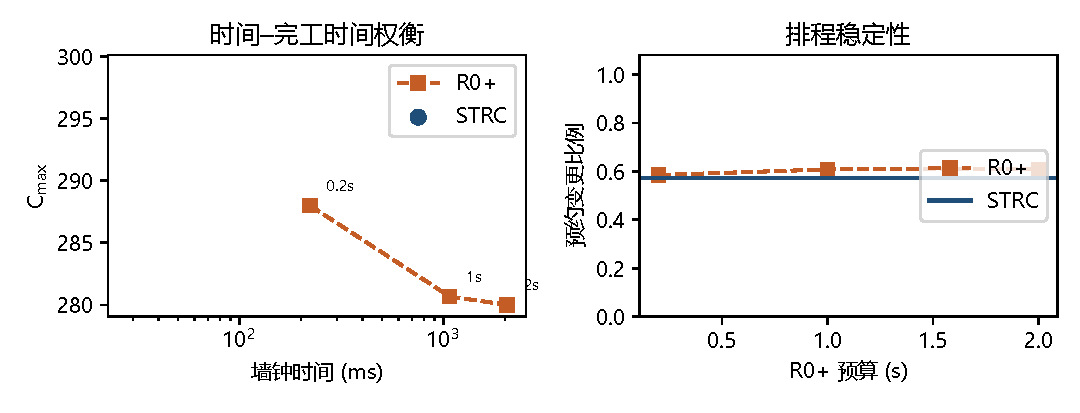
\includegraphics[width=\linewidth]{figures/fig_strc_e5_CN}
\caption{E5：不改写已结束占用的 R0+ 预算扫描与有界修复结果（\texttt{congested\_8x4x4}, \(3\) 个随机种子均值）。
左：算法耗时--\(C_{\max}\)，两条曲线不相交；右：占用改动比例，两法均约为 \(0.6\)。}
\Description{并排两幅图。左幅横轴为对数刻度的算法耗时、纵轴为完工时间：
不改写已结束占用的热启动全局重调度随预算略降，有界修复是左上方的一个单点，
两者不相交，全局重调度在每个预算点上都略低。右幅为占用改动比例，
两法均约为 0.6。}
\label{fig:e5}
\end{figure}

有界修复的完工时间在全部预算区间上均较差，但算法耗时低两至三个数量级（以第 1 级改路的 \(\MsRepairMed\)\,ms
对比 \(0.2\)--\(2\)\,s 预算，见图~\ref{fig:e5} 左）。这一耗时差来自单遍改路、不重新启动搜索，
\emph{并非}来自影响集划界；第~\ref{sec:cheap}~节以耗时相同的 RA 对照证实了这一点。
两者的改动比例同为 \ResFracRtwo\ 量级，改写量的比较见第~\ref{sec:cheap}~节与 RA 的对照。
要求毫秒量级响应时，有界修复能够恢复可行；允许秒级停机时，不改写已结束占用的热启动全局重调度在完工时间上占优。

本表的 R0+ 采用第~\ref{sec:vs_r0}~节的固定前缀解码，不改写已经结束的占用。
对已结束占用是否被改写的检查表明，小例与拥堵例各 \(9\) 个预算点的越界数均为 \(\RzeroPastLo\)；
当同一工件的后道工序已由车辆运出、前道工序仍需重新定时时，R0+ 强制沿用原车辆，只重规划 \(t_{\mathrm{now}}\) 之后的尾段，
从而保留已执行的空载前缀。有界修复在相同各格上的越界数同样为零。
因此，两者的完工时间差距中不包含「改写已经结束的占用」带来的部分，
剩余差距来自全局改派与改序相对单遍改路的优势。
因此，预约影响集的作用不体现在完工时间上，其适用场景是要求毫秒量级响应的恢复。

%% 标题里不放 \(\times\):它会进 PDF 书签,hyperref 无法处理数学模式。
\subsection{E6：扰动类型与划界对象的交叉}
\label{sec:e6}

E1--E3 只考察了走廊阻断一种扰动。本小节展开扰动类型这一维，在同一 \(\NPairs\) 对上另加
走廊通行变慢、车辆故障与机械臂故障三类，结果见表~\ref{tab:e6}。

\textbf{测量内容。} 划界方面，四类扰动均报告工序依赖图上影响域的规模、预约影响集的规模，以及后者是否包含前者。
修复方面，四类扰动均执行修复。B 类仍只改路：阻断把禁行窗写入预约表；通行变慢在窗内按倍率
\(\tau_{\mathrm{mult}}=2\) 降低通行进度，窗外仍按原 \(\tau\) 通行，走廊保持可通行。
A 类额外允许换车或改派，不改变加工顺序；是否扩大允许改写的范围不影响其动作集合。

\begin{table}[t]
\centering
\caption{E6 扰动类型 \(\times\) 划界对象（\(\NPairs\) 对/类，共 \(200\) 次测量；
其中两类 B 扰动按构造给出同一起点集，故\emph{独立}划界测量为 \(150\) 次，见正文第三点）。
\(|R^{\circ}|\) 为 \(t_{\mathrm{now}}\) 之后尚未结束的占用数。
「R1 为空」即按工序依赖图划界判该扰动无需重调度的格数。
末列不扩大范围：B 类为第 1 级改路，A 类为换车或改派。}
\label{tab:e6}
\small
\begin{tabular}{@{}llccccc@{}}
\toprule
扰动 & 类 & R1 为空 & 均 \(|U_{R1}|\) & 均 \(|\mathrm{Cl}|\)
 & \(\mathrm{Cl}/|R^{\circ}|\) & R2 可行 \\
\midrule
走廊阻断   & B & \(50/50\) & \(0.0\)  & \(64.4\) & \(0.92\) & \FeasESixBlock \\
走廊通行变慢 & B & \(50/50\) & \(0.0\)  & \(64.4\) & \(0.92\) & \FeasSlow \\
车辆故障   & A & \(0/50\)  & \(31.1\) & \(60.6\) & \(0.85\) & \FeasESixAgv \\
机械臂故障 & A & \(0/50\)  & \(42.8\) & \(65.9\) & \(0.94\) & \FeasESixRa \\
\bottomrule
\end{tabular}
\end{table}

四点结果。第一，\textbf{A/B 二分在 \(150\) 次\emph{独立}划界测量上无一例外}（两类 B 扰动共用同一起点集，见第三点）：两类 B 扰动按工序依赖图划界
全部为空，两类 A 扰动全部非空。第二，\textbf{在全部 \(100\) 次 A 类测量上
\(U_{R1}\subseteq\mathrm{Cl}\)}，即改用预约影响集划界在 A 类上不会\emph{遗漏}
工序依赖图已纳入的占用。包含在 \(\StrictlyLarger\) 格上是严格的，其余 \(13\) 格两者相等。
机械臂故障一行的包含\emph{按构造}成立：定义~\ref{def:seeds}(c) 的起点规则沿工件链
取整条后缀，而 \(U_{R1}\) 以 \(\theta=2\) 截断（第~\ref{sec:protocol}~节），故该行只验证实现与定义一致；
车辆故障一行的包含则是实测结果。
代价是允许改写的集合平均变大：车辆故障 \(31.1\to 60.6\)，机械臂故障 \(42.8\to 65.9\)。
第三，\textbf{通行变慢与阻断的划界结果逐格相同}，在全部 \(50\) 对上影响集规模一致。
这是因为二者的起点规则相同（与失效时窗重叠、尚未结束的占用），按构造给出同一个预约影响集；
该行表明按工序依赖图划界对通行变慢同样给出空范围。
第四，\textbf{修复方面四类扰动均全部可行}，逐类结果见表~\ref{tab:e6} 末列，通行变慢与阻断口径相同。
通行变慢只按倍率缩放与窗重叠部分的进度，走廊保持可通行，
因此它与「整段禁行后绕路」在物理上仍有区别；第 1 级改路即全部可行，未触发扩大范围。
车辆故障采用换车，机械臂故障采用改派。

\textbf{这张表也给出了影响集规模的实测}（注~\ref{rem:minimality}）。
走廊阻断下预约影响集覆盖 \(t_{\mathrm{now}}\) 之后尚未结束占用的约 \(\ClosureAliveFrac\)；
相对「把尚未结束的占用全部纳入改写」这一平凡上界只少纳入不足一成。
第~\ref{sec:e1}~节按全表统计的 \(\mathrm{Cl}/|R|\) 落在 \EoneCloLo--\EoneCloHi，
与此并不矛盾：全表还包含 \(t_{\mathrm{now}}\) 之前已执行完毕、不可改写的约一半占用。
就贡献而言，本节把 C1 与 C2 的结论从一种扰动推广到四种。

\subsection{E7：毫秒量级内的对照}
\label{sec:cheap}

E5 的对照是热启动种群搜索，预算 \(0.2\)--\(2\)\,s。仅以它为对照会留下一个问题：
\emph{「低两至三个数量级」这一结果，有多少来自预约影响集，又有多少只是因为对照方法耗时更长?}
本节补充耗时介于有界修复与热启动种群搜索之间的对照，并加入一个仅改变允许改写范围的对照。

\begin{itemize}[leftmargin=1.5em,itemsep=0.25em]
\item \textbf{RS（全局右移）。} 不改路径、不改指派、不改加工顺序，把未完成占用整体后推
一个延迟 \(\Delta\),\(\Delta\) 取到刚好让受阻走廊上所有可动的占用落到阻断窗之后。
不改写已经结束的占用（\(t^e\le t_{\mathrm{now}}\) 不可动），与 R2 相同；
由于是统一平移，所有时间间隔保持不变或变大，而全部约束都是「\(\ge\)」型，
无需重新路由即得可行解。它代表「\emph{不按影响集划界}」的一端，且完全不改路
（第~\ref{sec:rw_aor}~节）。
\item \textbf{RD（原染色体重解码）。} 保持机器指派与加工顺序，在已写入阻断的路由层上
执行与 R0+ 相同的固定前缀解码。它是本文实现中\emph{耗时最短的全局重算}；由于不改变染色体，其耗时比 R0+ 短，
改派与改序的自由度也更小。
\item \textbf{RA（不按影响集限制范围，但保留改路）。} 把 \(t_{\mathrm{now}}\) 之后\emph{尚未结束}的占用全部纳入改写，
再执行与 R2 \emph{完全相同}的改路重放。它代表「不按影响集划界」的另一端：与 RS 不同，它保留了
改路，因而与 R2 的唯一区别是允许改写的占用集合。两者使用同一套改路程序，都不改写已经结束的占用，且面对同一段阻断。
因此它是本文\emph{唯一}能单独隔离预约影响集作用的对照，两法之差不含改路程序、协议或实现的贡献。
RA 的允许改写集合已是最大，无需失败后扩大范围。
\end{itemize}

E3 比较的是两种\emph{不同}的划界对象（工序依赖图与预约影响集），而 RA 回答的问题是：
\emph{是否需要按影响集限制改写范围}。

\begin{table}[t]
\centering
\caption{E7 毫秒量级内对照（\(\NPairs\) 对，协议与 E3 相同：繁忙走廊单窗阻断、
\(t_{\mathrm{now}}=0.35\,C_{\max}^{0}\)、R2 不扩大范围）。四法均 \(\NPairs/\NPairs\) 可行。
「已结束占用越界」为改写了已结束占用的格数；「允许改写」为该方法纳入改写的占用占 \(t_{\mathrm{now}}\)
之后尚未结束占用的比例；末列为该方法对 R2 的 \(C_{\max}\) 胜负。RA 与 R2 只差允许改写哪些占用，
故这两行之差可全部归因于预约影响集。本表\emph{不可}与表~\ref{tab:e5} 直接比较，后者只含两个算例。}
\label{tab:cheap}
\small
\begin{tabular}{@{}lcccccc@{}}
\toprule
方法 & 已结束占用越界 & ms（中位）& 平均退化 & 改动比例 & 允许改写 & 对 R2 赢/平/输 \\
\midrule
RS 全局右移      & \ShiftBad     & \MsShift    & \(58.8\%\) & \ResFracShift    & ---   & \(7/16/27\) \\
RD 重解码        & \RedecodeBad  & \MsRedecode & \(49.0\%\) & \ResFracRedecode & ---   & \(22/14/14\) \\
RA 不按影响集划界 & \ShiftBad     & \MsAllFuture & \(49.9\%\) & \ResFracAllFuture & \(1.00\) & \(0/46/4\) \\
R2 有界修复      & \ShiftBad     & \MsCheapRtwo & \(49.8\%\) & \ResFracCheapRtwo & \ClosureShareMean & --- \\
\bottomrule
\end{tabular}
\end{table}

表~\ref{tab:cheap} 给出四条结果。

\textbf{其一，在给出可行方案的各法中，唯一比有界修复更快的是全局右移，
但它在完工时间与改动比例上均较差。}（按工序依赖图划界的 R1 更快，但其可行率仅为 \FeasRone，
不构成候选方法。）
RS 只需 \MsShift\,ms，约为 R2 的一半；代价是完工时间平均退化 \(58.8\%\)（R2 为
\(49.8\%\)），逐格对比为 \WinVsShift（R2 赢/平/输），且改动的占用更多
（\ResFracShift\ 对 \ResFracCheapRtwo），因为统一平移改变了每一条尚未结束占用的时刻。
若要使右移\emph{有选择}，即只推迟真正受影响的车辆而其余保持不变，就必须先
确定哪些占用受影响，而这正是本文划定的范围。\textbf{右移无需按影响集划界，正是因为
它放弃了选择。}

\textbf{其二，耗时最短的全局重算仍比有界修复慢。} RD 的耗时中位数为
\MsRedecode\,ms，是 R2 的 \RedecodeRatio\ 倍。这一结果与搜索配置无关：任何基于解码的搜索，
每评估一个候选至少需要一次解码。因此 E5 中「低两至三个数量级」\emph{并非}
由于对照方法耗时过长；将对照换成同一实现中耗时最短的全局重算，有界修复仍然更快。

\textbf{其三，在不改写已结束占用的前提下，RD 与 R2 的完工时间在本样本上无法区分，但 RD 改动更多。}
全表中 R2 对 RD 为 \WinVsRedecode（赢/平/输），平均退化 \(49.8\%\) 对 \(49.0\%\)。这一差别不显著：
配对差均值 \(+0.006\)，自助 \(95\%\) 区间 \([-0.007,\,0.019]\) 包含 \(0\);Wilcoxon 符号秩
双侧 \(p=0.12\)（非零差 \(36\) 格）；\(C_{\max}\) 比值均值 \(0.997\)，区间 \([0.988,\,1.007]\) 亦包含 \(1\)。
故两者在完工时间上未观察到差异。
RD 的已结束占用越界数为 \RedecodeBad：当后道工序已由车辆运出时，RD 强制沿用原车辆，只重规划决策时刻之后的尾段，
从而保留已执行的空载前缀。因此 RD 在逐格计数上的微弱优势来自同一染色体下全局改路相对单遍改路的优势，
而非改写已结束的占用。RD 的改动比例为 \ResFracRedecode，高于 R2 的
\ResFracCheapRtwo，即按影响集划界的一方改写更少。

\textbf{其四，改写量的减少只能由 R2 与 RA 的对比得出，且只体现为稳定性。} RA 与 R2 的唯一区别是允许改写的占用集合，因此这一对
结果直接给出按影响集划界的净收益。预约影响集平均只比平凡上界少纳入 \(1-\ClosureShareMean\)
的尚未结束占用（逐格为 \ClosureShareLo--\(1.00\)；在取值为 \(1.00\) 的 \(6\) 格上，影响集\emph{等于}
全部尚未结束占用，两法结果相同）。这不足一成的差别使改动比例从 \ResFracAllFuture\ 降至
\ResFracCheapRtwo：平均降低 \RAStabMean，中位数降低 \RAStabMed，逐格为 \RAStabWTL（R2 更稳/持平/更差），
Wilcoxon 符号秩双侧 \(p=\RAStabP\)。

剔除上述 \(6\) 个恒等格后为 \(44\) 格，逐格为 \RAStabWTLNet，平均降低 \RAStabMeanNet
（两种口径下 Wilcoxon 的非零差格数均为 \(32\)），即按 \NPairs\ 格报告的降幅偏保守。
降低的方向高度一致，但\emph{幅度不大}；在唯一的反例格上，R2 多改写了 \(0.007\)。
与此同时，两法的算法耗时几乎相同（\MsCheapRtwo\ 对 \MsAllFuture\,ms），
完工时间也几乎相同（比值均值 \RACmaxRatio，逐格 R2 赢/平/输为 \WinVsAllFuture，从未更差，
最优的一格为 \RACmaxLo）。

上述三项结果需要合并解读。\textbf{耗时相同，说明毫秒量级的响应来自单遍改路、不重新启动搜索，而非来自预约影响集
（结果见表~\ref{tab:cheap}；单遍改路本身是既有做法，见表~\ref{tab:position}）。
完工时间相同，说明影响集不是一种优化手段。
改动比例显著更低，说明划界实现的正是命题~\ref{prop:outside} 所保证的性质：集外占用的走廊、时段与车辆保持不变。}
影响集的作用在于\emph{标明哪些占用无需改写}。
影响集排除的占用越多，降幅越大；但被排除的占用本身只能解释
\(\ResFracAllFuture-\ResFracCheapRtwo\) 这一差距的一部分，其余来自允许改写集合缩小后改路结果的变化。
在影响集接近全部尚未结束占用的算例上（\texttt{congested\_8x4x4}，允许改写占比 \(0.94\)），
降幅仅为 \(0.010\)；而在排除较多占用的算例上(\texttt{S8x4x4\_mid},\(0.91\))，降幅达 \(0.118\)。
% selfcheck:allow-num 0.91 为该算例的允许改写占比,与 \ScaleCloAliveHi(E8 档均值上界)同值不同源
两个算例只能说明方向，逐格分布见下文。

下面将这一方向整理为一条事后分档规则。图~\ref{fig:worth} 以允许改写占比
\(\mathrm{Cl}/|R^{\circ}|\) 为横轴、RA 相对 R2 的改动比例降幅为纵轴，画出 \(\NPairs\) 对。
在本样本上取 \(\mathrm{Cl}/|R^{\circ}|\ge\WorthThresh\)：该线以上 \WorthHighN\ 格平均降幅
\WorthHighMean，以下 \WorthLowN\ 格平均降幅 \WorthLowMean；
占比超过 \(\WorthVanish\) 的各格降幅均为零，但成因有两种：占比恰为 \(1.00\) 的 \(6\) 格上，
影响集等于全部尚未结束占用，两法\emph{恒等}；其余各格占比不足 \(1.00\) 而降幅已为 \(0\)，
属于实测结果而非恒等。
该阈值在本样本上选定，用于回答「何时按影响集划界仍有收益」，不作外推，
也不同于影响集规模的结构预测（第~\ref{sec:e4}~节）。

\begin{figure}[t]
\centering
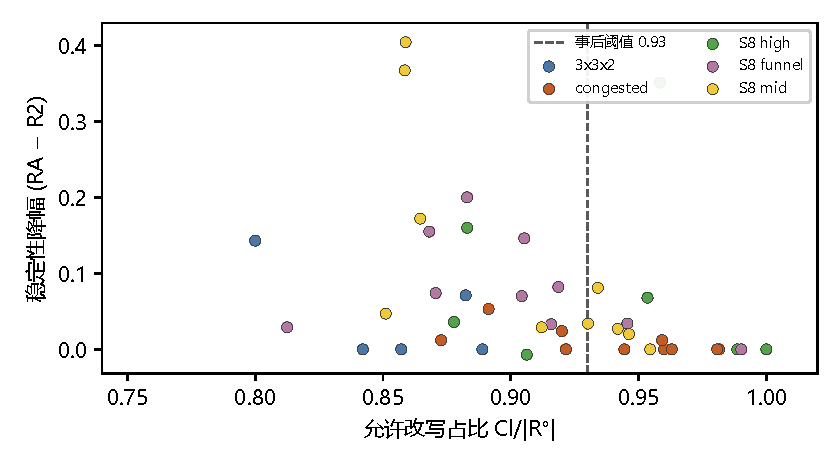
\includegraphics[width=0.92\linewidth]{figures/fig_strc_worth_CN}
\caption{E7 事后规则：允许改写占比与稳定性降幅（\(\NPairs\) 对，R2 对 RA）。
虚线为样本内阈值 \(\WorthThresh\)；纵轴为正表示按影响集划界后改动比例更低。}
\Description{散点图，横轴为预约影响集占尚未结束占用的比例，纵轴为不按影响集划界相对划界多改的占用比例，
五个算例用不同颜色区分，一条竖虚线标在 \WorthThresh。点大致从左上到右下。}
\label{fig:worth}
\end{figure}

综合四种方法的结果：在「不改写已经结束的占用」且「响应须在毫秒量级」两个约束下，
\textbf{按影响集划界的净收益只体现在改写量上。}
\textbf{在速度与完工时间相同的条件下，不划界需多改写约 \(6\) 个百分点的占用（相对增加约 \(12\%\)）}，
而划界\emph{不}带来速度或完工时间上的优势。
放宽耗时约束后，更短的完工时间仍来自热启动搜索（第~\ref{sec:e5}~节），
但其耗时已超出毫秒量级。

